\documentclass[10pt,a4paper, margin=1in]{article}
\usepackage{fullpage}
\usepackage{amsfonts, amsmath, pifont}
\usepackage{amsthm}
\usepackage{graphicx}
\usepackage{float}
\usepackage{minted}
\usepackage{tkz-euclide}
\usepackage{tikz}
\usepackage{pgfplots}
\pgfplotsset{compat=1.13}

\usepackage{geometry}
 \geometry{
 a4paper,
 total={210mm,297mm},
 left=10mm,
 right=10mm,
 top=10mm,
 bottom=10mm,
 }
 % Write both of your names here. Fill exxxxxxx with your ceng mail address.
 \author{
  Geçit, Emre\\
  \texttt{e2521581@ceng.metu.edu.tr}
  \and
  Yancı, Baran\\
  \texttt{e2449015@ceng.metu.edu.tr}
}

\title{CENG 384 - Signals and Systems for Computer Engineers \\
Spring 2023 \\
Homework 2}
\begin{document}
\maketitle



\noindent\rule{19cm}{1.2pt}

\begin{enumerate}

\item %write the solution of q1
    \begin{enumerate}
    % Write your solutions in the following items.
    \item %write the solution of q1a
    \begin{align*}
        y(t) & = x(t) - 5 \dot{y}(t) \\
    \end{align*}
    \item %write the solution of q1b
    \begin{align*}
        y(t) & = (e^{-t} + e^{-3t})u(t) - 5 \dot{y}(t) \\
        y(t) + 5 \dot{y}(t) & = (e^{-t} + e^{-3t})u(t) \\
        y(t) & = y_p(t) + y_h(t) \\
        y_p(t) & = Ke^{-t}u(t) + Le^{-3t}u(t) \\
        Ke^{-t}u(t) + Le^{-3t}u(t) + 5 (-Ke^{-t}u(t) -3Le^{-3t}u(t)) & = (e^{-t} + e^{-3t})u(t) \\
        Ke^{-t}u(t) + Le^{-3t}u(t) - 5Ke^{-t}u(t) - 15Le^{-3t}u(t) & = (e^{-t} + e^{-3t})u(t) \\
        e^{-t}u(t) (K - 5K) + e^{-3t}u(t) (L - 15L) & = (e^{-t} + e^{-3t})u(t) \\
        K - 5K & = 1 \\
        K & = - 1/4 \\
        L - 15L & = 1 \\
        L & = - 1/14 \\
        y_p(t) & = \frac{-1}{4}e^{-t}u(t) + \frac{-1}{14}e^{-3t}u(t) \\
        y_h(t) & = c_1e^{\alpha t} \\
        c_1e^{\alpha t} + 5\alpha c_1e^{\alpha t} & = 0 \\
        c_1 + 5\alpha c_1 & = 0 \\
        \alpha & = \frac{-1}{5} \\
        y_h(t) & = c_1e^{\frac{-1}{5}t} \\
        y(t) & = y_p(t) + y_h(t) \\
        & = \frac{-1}{4}e^{-t}u(t) + \frac{-1}{14}e^{-3t}u(t) + c_1e^{\frac{-1}{5}t} \\
        y(0) & = 0 \\
        0 & = \frac{-1}{4} + \frac{-1}{14} + c_1 \\
        c_1 & = \frac{9}{28} \\
        y(t) & = \frac{-1}{4}e^{-t}u(t) + \frac{-1}{14}e^{-3t}u(t) + \frac{9}{28}e^{\frac{-1}{5}t} \\
    \end{align*}
    \end{enumerate}

\item %write the solution of q2  
	\begin{enumerate}
    % Write your solutions in the following items.
    \item %write the solution of q2a
    \begin{align*}
        y[n] & = x[n] * h[n] \\
        & = \sum_{k=0}^{n} x[k]h[n-k] \\
        & = \sum_{k=0}^{n} \left(2\delta [k] + \delta [k + 1]\right) \left(\delta [n-(1+k)] + 2\delta [n+1-k]\right) \\
        & = 2\sum_{k=0}^{n} \delta [k] \delta [n-(1+k)] + 4\sum_{k=0}^{n} \delta [k] \delta [n+1-k] + \sum_{k=0}^{n} \delta [k + 1] \delta [n-(1+k)] + 2\sum_{k=0}^{n} \delta [k + 1] \delta [n+1-k] \\
        & = 2\delta\left[n - 1\right] + 4\delta\left[n + 1\right] + \delta\left[n\right] + 2\delta\left[n + 2\right] \\
    \end{align*}

    \begin{center}
        \begin{tikzpicture}
            \begin{axis}[ xlabel=$n$, ylabel=$y$, axis x line=center, axis y line = center, xmin=-3.5, xmax=3.5, ymin=-6, ymax=6]
                \addplot+[ycomb,mark=triangle,mark options={rotate=0}] plot coordinates {(-2, 2) (-1, 4) (0, 1) (1, 2)};
            \end{axis}
        \end{tikzpicture}
    \end{center}

    \item %write the solution of q2b
    % TODO: this feels wrong
    \begin{align*}
        y(t) & = \frac{dx(t)}{dt} * h(t) \\
        & = \frac{d}{dt}\left(u(t-1) + u(t+1)\right) * e^{-t} \sin (t)u(t) \\
        & = \left(\delta(t-1) + \delta(t+1)\right) * e^{-t} \sin (t)u(t) \\
        & = \int_{-\infty}^{\infty} \left(\delta(\tau-1) + \delta(\tau+1)\right) e^{-t - \tau} \sin (t - \tau) d\tau \\
        & = \int_{-\infty}^{\infty} \delta(\tau-1)e^{-t - \tau} \sin (t - \tau) d\tau + \int_{-\infty}^{\infty} \delta(\tau+1) e^{-t - \tau} \sin (t - \tau) d\tau \\
        & = e^{-t - 1} \sin (t - 1)u(t -1) + e^{-t + 1} \sin (t + 1)u(t + 1) \\
    \end{align*}
    \end{enumerate}

\item %write the solution of q3
    \begin{enumerate}
    % Write your solutions in the following items.
    \item %write the solution of q3a

    % @y4nci: see https://odtuclass2022s.metu.edu.tr/pluginfile.php/523917/mod_resource/content/14/week_4.html#convolution-operation-in-continuous-time exercise 4.1

    \begin{align*}
        y(t) & = x(t) * h(t) \\
        & = \int_{-\infty}^{\infty} x(\tau) h(t - \tau) d\tau \\
        & = \int_{-\infty}^{\infty} x(t - \tau) h(\tau) d\tau \\
        & = \int_{-\infty}^{\infty} e^{-(t - \tau)} e^{-2\tau} d\tau \\
        & = \int_{0}^{t} e^{-(t - \tau)} e^{-2\tau} d\tau \\
        & = e^{-t} \int_{0}^{t} e^{\tau} d\tau \\
        & = e^{-t} \left(1 - e^{-t}\right)u(t) \\
    \end{align*}
    \item %write the solution of q3b
    \begin{align*}
        y(t) & = x(t) * h(t) \\
        & = \int_{-\infty}^{\infty} x(\tau) h(t - \tau) d\tau \\
        & = \int_{-\infty}^{\infty} x(t - \tau) h(\tau) d\tau \\
        & = \int_{-\infty}^{\infty} \left(u(t - \tau) - u(t - (\tau + 1))\right) e^{3\tau} d\tau \\
        & = \int_{-\infty}^{\infty} u(t - \tau) e^{3\tau} d\tau - \int_{-\infty}^{\infty} u(t - (\tau + 1)) e^{3\tau} d\tau \\
        & = \int_{-\infty}^{t} e^{3\tau} d\tau - \int_{-\infty}^{t - 1} e^{3\tau} d\tau \\
        & = \frac{e^{3t}}{3} - \frac{e^{3t - 3}}{3}\\
    \end{align*}
    \end{enumerate}

\item %write the solution of q4
    \begin{enumerate}   
    % Write your solutions in the following items.
    \item %write the solution of q4a
    \begin{align*}
        y[n] - y[n - 1] - y[n - 2] & = 0\\
        y[n] & = y[n - 1] + y[n - 2]\\
        y[2] & = y[1] - y[0] = 2\\
        y[3] & = y[2] - y[1] = 3\\
        y[4] & = y[3] - y[2] = 5\\
        y[5] & = y[4] - y[3] = 8\\
        & ... \\
    \end{align*}

    It is the Fibonacci sequence.

    \begin{align*}
        y[n] & = \frac{(1 + \sqrt{5})^n - (1 - \sqrt{5})^n}{2^n \sqrt{5}} \\
    \end{align*}

    \item %write the solution of q4b
    \begin{align*}
        y^{(3)}(t) - 6y''(t) + 13y'(t) - 10y(t) & = 0\\
        % y(y2 -7y1 + 10y0) + (y2 +3y1 -10y0) => y(y-5)(y-2) + (y+5)(y-2)
        K^3 - 6K^2 + 13K - 10 & = 0\\
        K(K - 5)(K - 2) + (K + 5)(K - 2) & = 0\\
        (K - 2) (K^2 - 4K + 5) & = 0\\
        & \\
        K & = 2, 2 - j, 2 + j \\
    \end{align*}
    \begin{align*}
        y_h(t) & = c_1e^{2t} + c_2e^{(2 + j)t} + c_3e^{(2 - j)t} \\
        y_h(t) & = c_1e^{2t} + c_2\left(e^{2t}\cos(t) + je^{2t}\sin(t)\right) + c_3\left(e^{2t}\cos(t) - je^{2t}\sin(t)\right) \\
        y_h(t) & = c_1e^{2t} + c_2e^{2t}\cos(t) + c_3e^{2t}\cos(t) + c_2je^{2t}\sin(t) - c_3je^{2t}\sin(t) \\
        y_h(t) & = c_1e^{2t} + (c_2 + c_3) e^{2t}\cos(t) + j(c_2 - c_3)e^{2t}\sin(t)\\
        y_h(t) & = C_1e^{2t} + C_2e^{2t}\cos(t) + C_3e^{2t}\sin(t)\\
    \end{align*}
    \begin{align*}
        y''(0) & = 3\\
        & = 4C_1 + 3C_2 + 4C_3\\
        y'(0) & = 1.5\\
        & = 2C_1 + 2C_2 + C_3\\
        y(0) & = 1\\
        & = C_1 + C_2\\
        & \\
        C_1 & = 2\\
        C_2 & = -1\\
        C_3 & = -0.5\\
        & \\
        y_h(t) & = 2e^{2t} - e^{2t}\cos(t) - \frac{1}{2}e^{2t}\sin(t)\\
    \end{align*}
    \end{enumerate}

\item %write the solution of q5
    % TODO: feels wrong, needs review
    \begin{enumerate}
    % Write your solutions in the following items.
    \item %write the solution of q5a
    \begin{align*}
        y''(t) + 5y'(t) + 6y(t) & = \cos(5t)\\
        & = \frac{e^{j5t} - e^{-j5t}}{2}\\
        & = \frac{e^{j5t}}{2} - \frac{e^{-j5t}}{2}\\
    \end{align*}
    \begin{align*}
        y_p(t) & = c_1e^{j5t} + c_2e^{-j5t}\\
    \end{align*}
    \begin{align*}
        -25c_1e^{j5t} - 25c_2e^{-j5t} + 25jc_1e^{j5t} - 25jc_2e^{-j5t} + 6c_1e^{j5t} + 6c_2e^{-j5t} & = \frac{e^{j5t}}{2} - \frac{e^{-j5t}}{2}\\
        e^{j5t} \left(-19c_1 + 25jc_1\right) + e^{-j5t} \left(-19c_2 - 25jc_2\right) & = \frac{e^{j5t}}{2} - \frac{e^{-j5t}}{2}\\
    \end{align*}
    \begin{align*}
        \left(-19c_1 + 25jc_1\right) & = \left(-19c_2 - 25jc_2\right) = \frac{1}{2}\\
        & \\
        c_1 & = \frac{1}{50j - 38} \\
        c_2 & = \frac{-1}{50j + 38} \\
        y_p(t) & = \frac{1}{50j - 38}e^{j5t} - \frac{1}{50j + 38}e^{-j5t}\\
    \end{align*}
    \item %write the solution of q5b
    \begin{align*}
        y''(t) + 5y'(t) + 6y(t) & = 0\\
        K^2 + 5K + 6 & = 0\\
        K & = -3, -2\\
        & \\
        y_h(t) & = c_1e^{-3t} + c_2e^{-2t}\\
    \end{align*}
	\item %write the solution of q5c
    \begin{align*}
        y(t) & = y_p(t) + y_h(t)\\
        & = \frac{1}{50j - 38}e^{j5t} - \frac{1}{50j + 38}e^{-j5t} + c_1e^{-3t} + c_2e^{-2t}\\
    \end{align*}
    \begin{align*}
        y(0) = y'(0) = 0& \\
        \frac{1}{50j - 38} - \frac{1}{50j + 38} + c_1 + c_2 & = 0\\
        \frac{5j}{50j - 38} + \frac{5j}{50j + 38} - 3c_1 - 2c_2 & = 0\\
    \end{align*}
    \begin{align*}
        c_1 & = \frac{3}{34} \\
        c_2 & = \frac{-2}{29} \\
    \end{align*}
    \begin{align*}
        y(t) & = \frac{1}{50j - 38}e^{j5t} - \frac{1}{50j + 38}e^{-j5t} + \frac{3}{34}e^{-3t} - \frac{2}{29}e^{-2t}\\
    \end{align*}
    \end{enumerate}    
    
\item %write the solution of q6
    \begin{enumerate}
    % Write your solutions in the following items.
    \item %write the solution of q6a
    \begin{align*}
        w[n] - \frac{1}{2}w[n - 1] & = x[n]\\
        w[n] & = 0,  \forall n < 0 \\
        w[0] - \frac{1}{2}w[-1] & = x[0]\\
        w[0] & = x[0]\\
        w[1] - \frac{1}{2}w[0] & = x[1]\\
        w[1] & = x[1] + \frac{1}{2}x[0]\\
        w[2] - \frac{1}{2}w[1] & = x[2]\\
        w[2] & = x[2] + \frac{1}{2}x[1] + \frac{1}{4}x[0]\\
        &...\\
        w[n] & = \sum_{k = 0}^{n} 2^{-k}x[n - k]\\
        & \\
        h_0[n] & = \sum_{k = 0}^{n} 2^{-k}\delta[n - k]\\
        & = 2^{-n} & (\delta[n-k] = 0 \text{ for } k != n)\\
    \end{align*}
    \item
    If we feed the first system with the unit impulse, we get $h_0[n]$. If we feed the second system with $h_0[n]$, we get
    \begin{align*}
        h[n] &= \sum_{k = 0}^{n} 2^{-k}2^{-n+k} \\
        &= \sum_{k = 0}^{n} 2^{-n} \\
        &= (n+1) * 2^{-n} \\
    \end{align*}
    \item \begin{align*}
        y[n] = x[n] * h[n] \\
        &= \sum_{k = -\infty}^{\infty} x[n-k]h[k] \\
        &= \sum_{k = 0}^{\infty} x[n-k]h[k] & (h[k] = 0 \text{ for } k < 0)\\
        &= \sum_{k = 0}^{\infty} x[k]*(n+1) * 2^{k-n} \\
    \end{align*}
    \end{enumerate}
    
\item The code used to generate the plots is at the end of the answer.

\begin{figure}[H]    
    \centering
    \caption{Original Signal}
    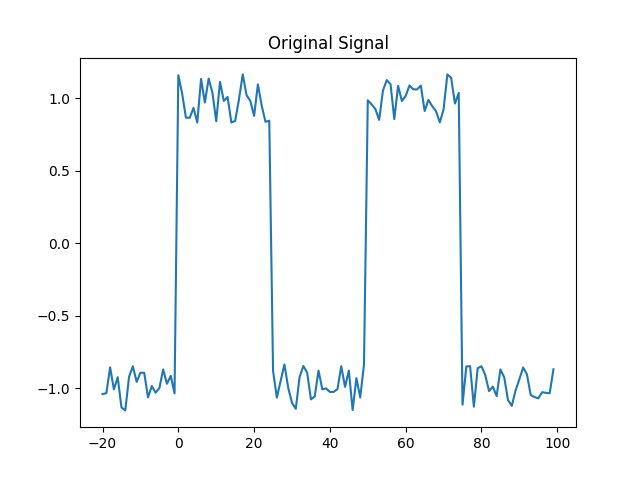
\includegraphics[width=0.4\linewidth]{images/original.png}
\end{figure}
\begin{enumerate}
    \item The effect of convoluting with $\delta[n-5]$ is to shift the signal by 5 units to the right.
\begin{figure}[H]
    \centering
    \caption{Convolution with $h[n] = \delta[n-5]$}
    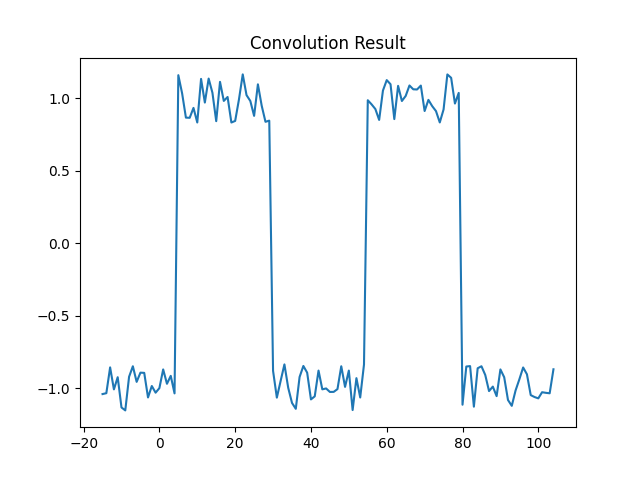
\includegraphics[width=0.4\linewidth]{images/convolution.png}
\end{figure}
    \item By convolving a signal with an n-point moving average filter, it is possible to effectively smooth the abrupt transitions or edges in the signal, as well as attenuate any unwanted noise present in the signal.
\begin{figure}[H]
    \centering
    \caption{Convolution with the moving average filter, N = 3}
    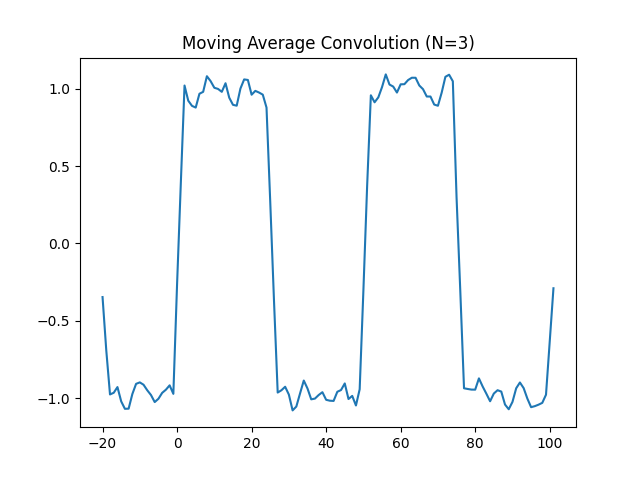
\includegraphics[width=0.4\linewidth]{images/moving_average_3.png}
\end{figure}
\begin{figure}[H]
    \centering
    \caption{Convolution with the moving average filter, N = 5}
    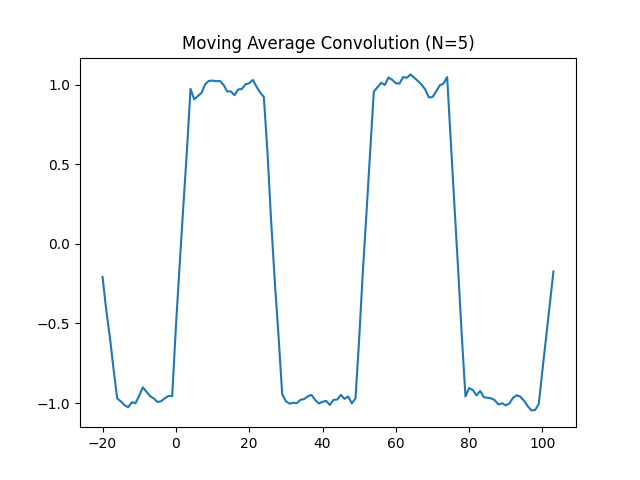
\includegraphics[width=0.4\linewidth]{images/moving_average_5.png}
\end{figure}
\begin{figure}[H]
    \centering
    \caption{Convolution with the moving average filter, N = 10}
    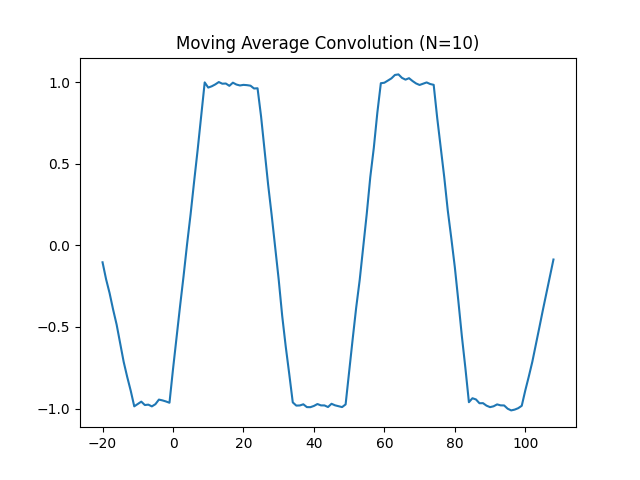
\includegraphics[width=0.4\linewidth]{images/moving_average_10.png}
\end{figure}
\begin{figure}[H]
    \centering
    \caption{Convolution with the moving average filter, N = 20}
    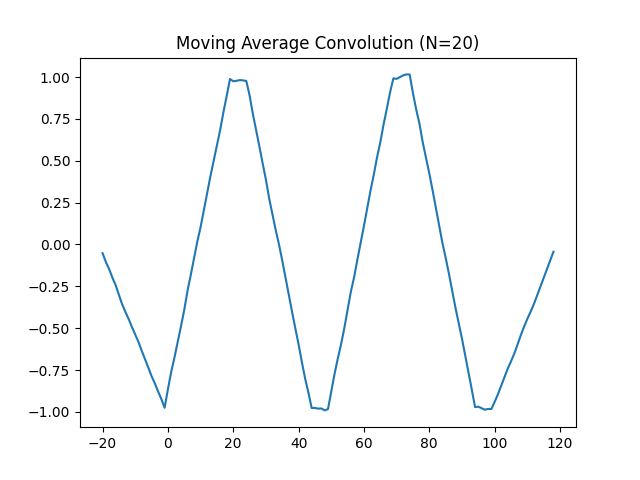
\includegraphics[width=0.4\linewidth]{images/moving_average_20.png}
\end{figure}

\begin{figure}
    \caption{Python Code}
    \inputminted{python}{hw2.py}
\end{figure}
    \end{enumerate}

\end{enumerate}


\end{document}

